% Copyright 2004 by Till Tantau <tantau@users.sourceforge.net>.
%
% In principle, this file can be redistributed and/or modified under
% the terms of the GNU Public License, version 2.
%
% However, this file is supposed to be a template to be modified
% for your own needs. For this reason, if you use this file as a
% template and not specifically distribute it as part of a another
% package/program, I grant the extra permission to freely copy and
% modify this file as you see fit and even to delete this copyright
% notice. 

\documentclass{beamer}

\usepackage[dutch]{babel}
\usepackage{float}
% There are many different themes available for Beamer. A comprehensive
% list with examples is given here:
% http://deic.uab.es/~iblanes/beamer_gallery/index_by_theme.html
% You can uncomment the themes below if you would like to use a different
% one:
%\usetheme{AnnArbor}
%\usetheme{Antibes}
%\usetheme{Bergen}
%\usetheme{Berkeley}
%\usetheme{Berlin}
%\usetheme{Boadilla}
%\usetheme{boxes}
%\usetheme{CambridgeUS}
%\usetheme{Copenhagen}
%\usetheme{Darmstadt}
\usetheme{default}
%\usetheme{Frankfurt}
%\usetheme{Goettingen}
%\usetheme{Hannover}
%\usetheme{Ilmenau}
%\usetheme{JuanLesPins}
%\usetheme{Luebeck}
%\usetheme{Madrid}
%\usetheme{Malmoe}
%\usetheme{Marburg}
%\usetheme{Montpellier}
%\usetheme{PaloAlto}
%\usetheme{Pittsburgh}
%\usetheme{Rochester}
%\usetheme{Singapore}
%\usetheme{Szeged}
%\usetheme{Warsaw}

\beamertemplatenavigationsymbolsempty


\title{A Model for \\Experiment Setups on \\FPGA Development Boards}

% A subtitle is optional and this may be deleted
% \subtitle{Optional Subtitle}

\author{Matthijs Bos}
% - Give the names in the same order as the appear in the paper.
% - Use the \inst{?} command only if the authors have different
%   affiliation.

\institute[Universities of Somewhere and Elsewhere] % (optional, but mostly needed)
{
  BSc Informatica\\
  Universiteit van Amsterdam (UvA)\\
  \vspace{1.5em}
  Begeleiders:\\
  \vspace{0.3em}
  A. van Inge\\
  T. Walstra}
% - Use the \inst command only if there are several affiliations.
% - Keep it simple, no one is interested in your street address.

\date{30 augustus 2016}
% - Either use conference name or its abbreviation.
% - Not really informative to the audience, more for people (including
%   yourself) who are reading the slides online

% \subject{Theoretical Computer Science}
% This is only inserted into the PDF information catalog. Can be left
% out. 

% If you have a file called "university-logo-filename.xxx", where xxx
% is a graphic format that can be processed by latex or pdflatex,
% resp., then you can add a logo as follows:

% \pgfdeclareimage[height=0.4cm]{university-logo}{logoUvA_nl_xl.pdf}
% \logo{\pgfuseimage{university-logo}}

% Delete this, if you do not want the table of contents to pop up at
% the beginning of each subsection:
% \AtBeginSubsection[]
% {
%   \begin{frame}<beamer>{Inhoud}
%     \tableofcontents[currentsection,currentsubsection]
%   \end{frame}
% }

% Let's get started
\begin{document}

\begin{frame}
\let\thefootnote\relax
  \titlepage
\end{frame}

\begin{frame}{Inhoud}
  \tableofcontents
  % - introductie: jezelf voorstellen. Thesis statement, vertel kort wat je scriptie inhoudt, je abstract bij wijze van. 
  % - achtergrond FPGA's
  % - problem statement. Belangrijk om je scope te definieren en tot de kern te komen.
  % - overzicht model, niet per se de hele ontwikkeling, maar wel de belangrijkste aspecten.
  % - Resultaten: implementatie en evaluatie. Laat eventueel zien dat je hier in bent te kort geschoten.
  % - conclusie
  % - Future work
\end{frame}

% Section and subsections will appear in the presentation overview
% and table of contents.
\section{Introductie}

\subsection{Achtergrond}

\begin{frame}{FPGA's}{Field Programmable Gate Array}
    
    \begin{figure}
        \centering
        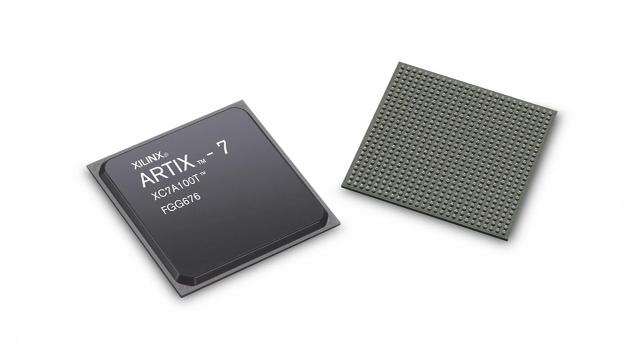
\includegraphics[width=\textwidth]{img/artix7}
    \end{figure}
\end{frame}

\subsection{Probleemstelling}

% \begin{frame}{Probleemstelling}{Experimenteren met digitale logica middels FPGA's}
%   \begin{figure}
%       \centering
%       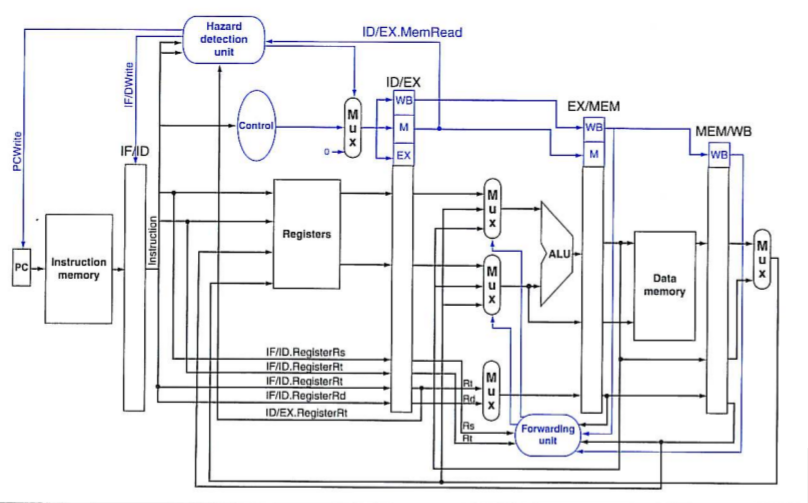
\includegraphics[width=\textwidth]{img/hpmips}
%   \end{figure}
% \end{frame}

\begin{frame}{Probleemstelling}{Experimenteren met digitale logica middels FPGA's}
  \begin{itemize}
    \item Eerstejaars studenten computerarchitectuur en organisatie
    \vspace{1em}
    \item Experimentele analyse complexe aspecten
    \vspace{1em}
    \item FPGA's als fysieke component
    \vspace{1em}
    \item kant-en-klare experimentele opstellingen
      \begin{itemize}
          \item Eenvoudige ontwikkeling
      \end{itemize}
    \vspace{0.7em}
    \item Interactie middels PC
  \end{itemize}
\end{frame}

\subsection{Onderzoeksvragen}
\begin{frame}{Onderzoeksvragen}{Experimenteren met digitale logica middels FPGA's}
\begin{enumerate}
    \item Hoe kan het ontwikkelproces worden aangepast?
        \begin{itemize}
            \item Hergebruik componenten
            \item Afscherming specialistische aspecten
        \end{itemize}
    \vspace{2em}
    \item Hoe kunnen FPGA's worden ingezet tijdens de uitvoering van experimenten?
        \begin{itemize}
            \item Technische complexiteit verbergen
            \item Implementatie niet vereist
        \end{itemize}
\end{enumerate}
\end{frame}


\section{Model}

\subsection{Interactie}
\begin{frame}{Model: Interactie}{Afscheiding besturende logica}
\begin{figure}[h]
    \centering
    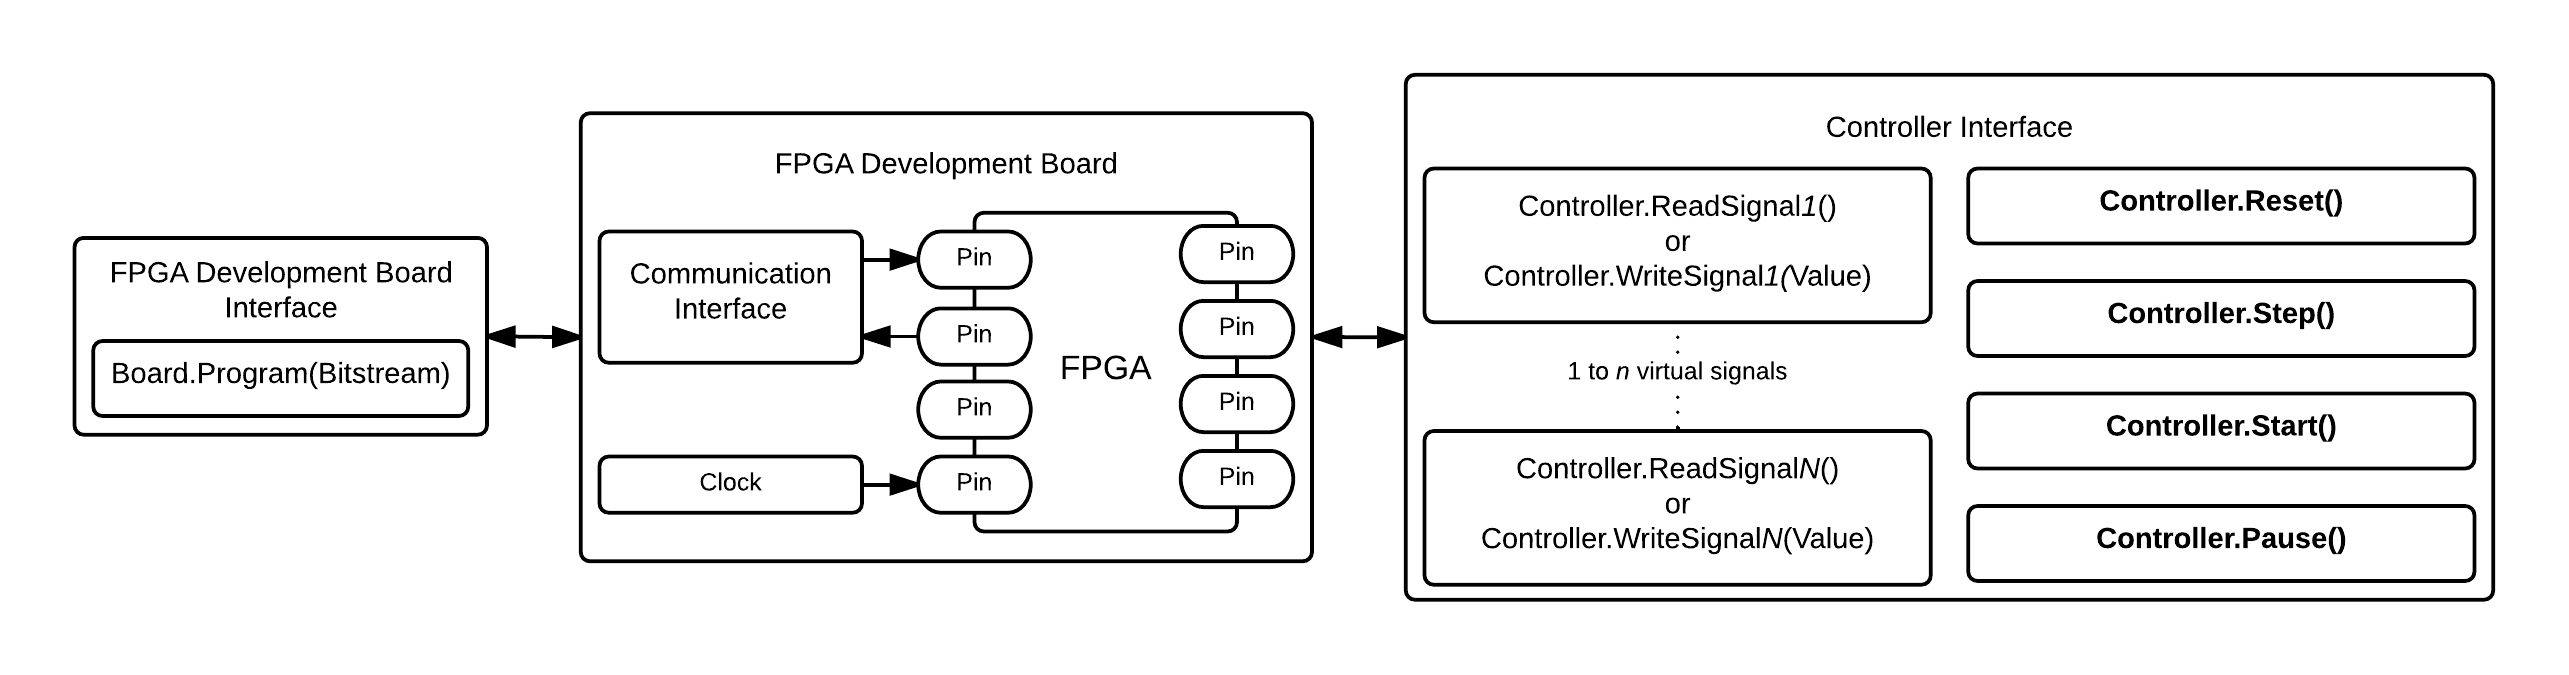
\includegraphics[width=\textwidth]{img/overview-control}
\end{figure}
\begin{figure}[h]
    \centering
    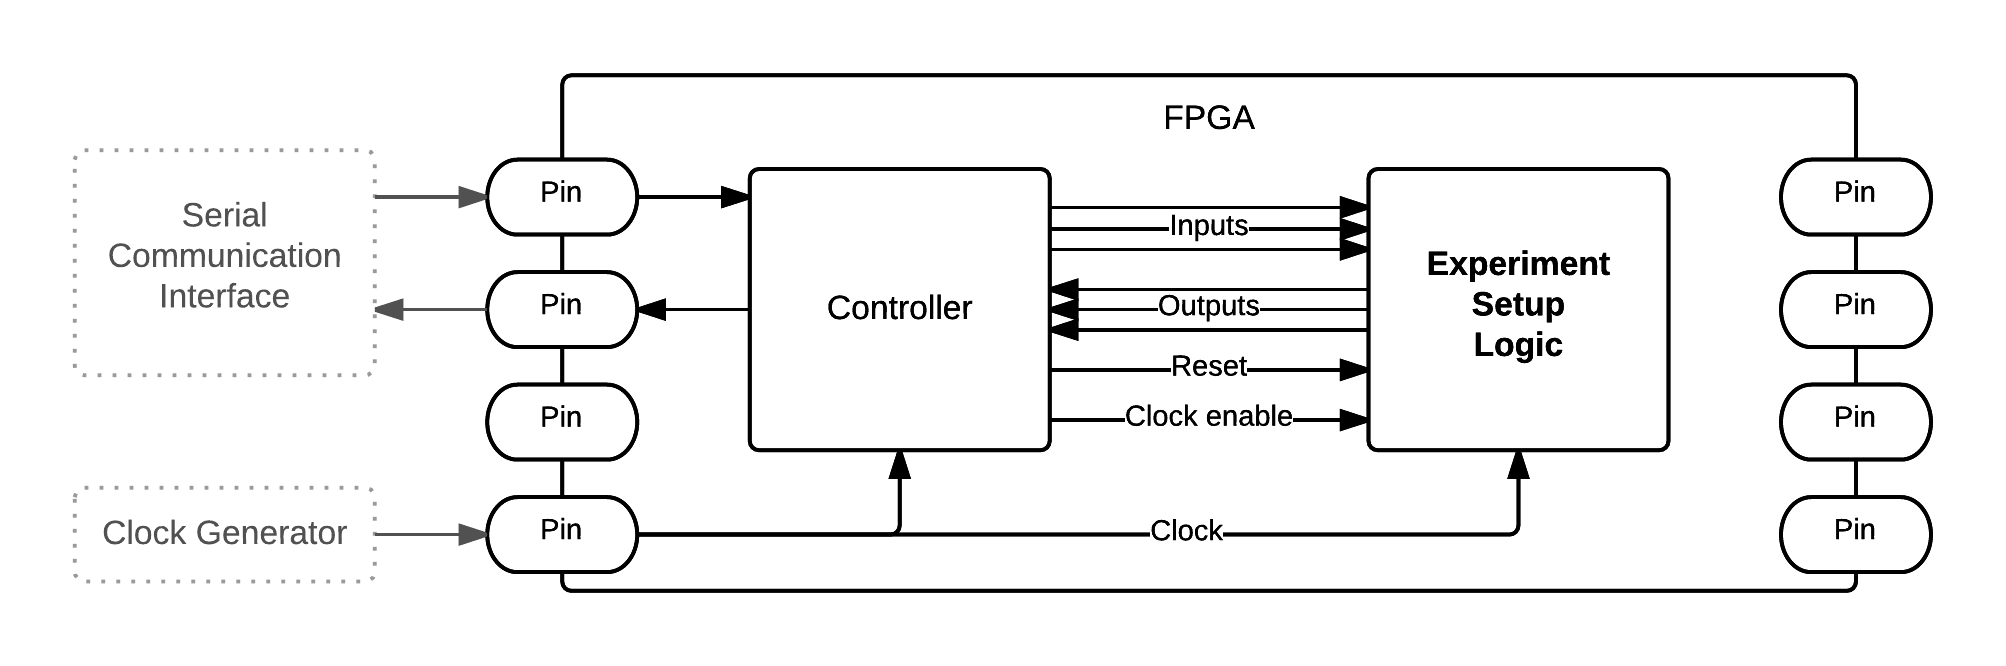
\includegraphics[width=\textwidth]{img/fpga-control}
\end{figure}
\end{frame}

\subsection{Generalisatie}
\subsubsection{Adresruimte}
\begin{frame}{Model: Generalisatie koppelingen}
\begin{block}{Adresruimte}
\begin{itemize}
    \item Reeks geheugenplekken
    \item Twee operaties:
        \begin{itemize}
            \item \texttt{Read(Address)}
            \item \texttt{Write(Address, Value)}
        \end{itemize}
\end{itemize}
\end{block}
\begin{figure}[h]
    \centering
    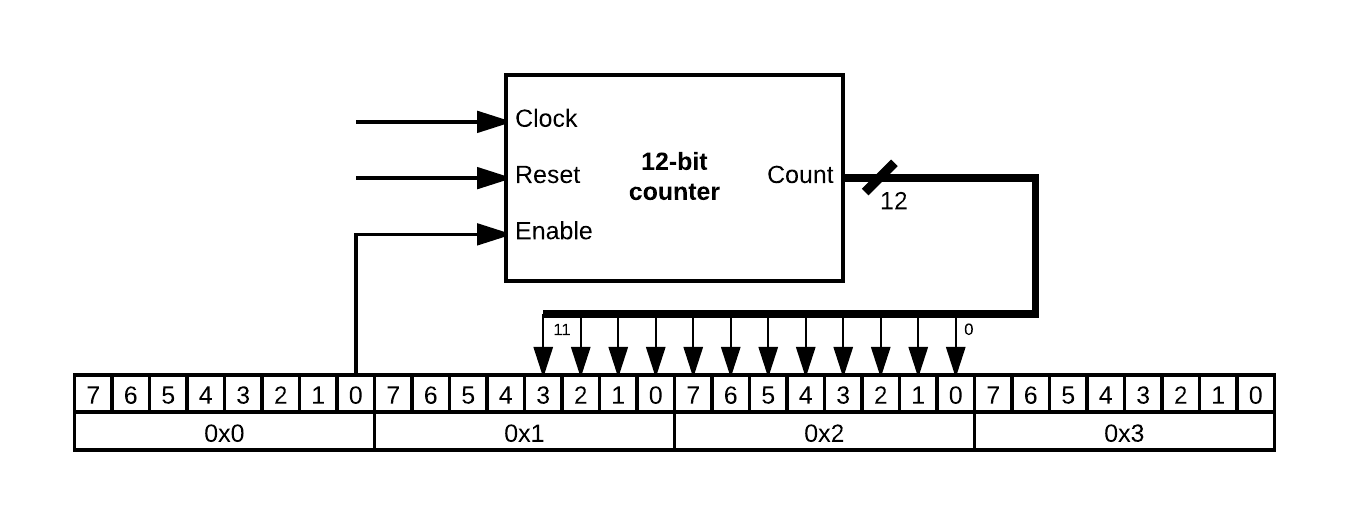
\includegraphics[width=\textwidth]{img/signal-address-projection}
\end{figure}
\end{frame}

\begin{frame}{Model: Generalisatie koppelingen}
\begin{figure}[h]
    \centering
    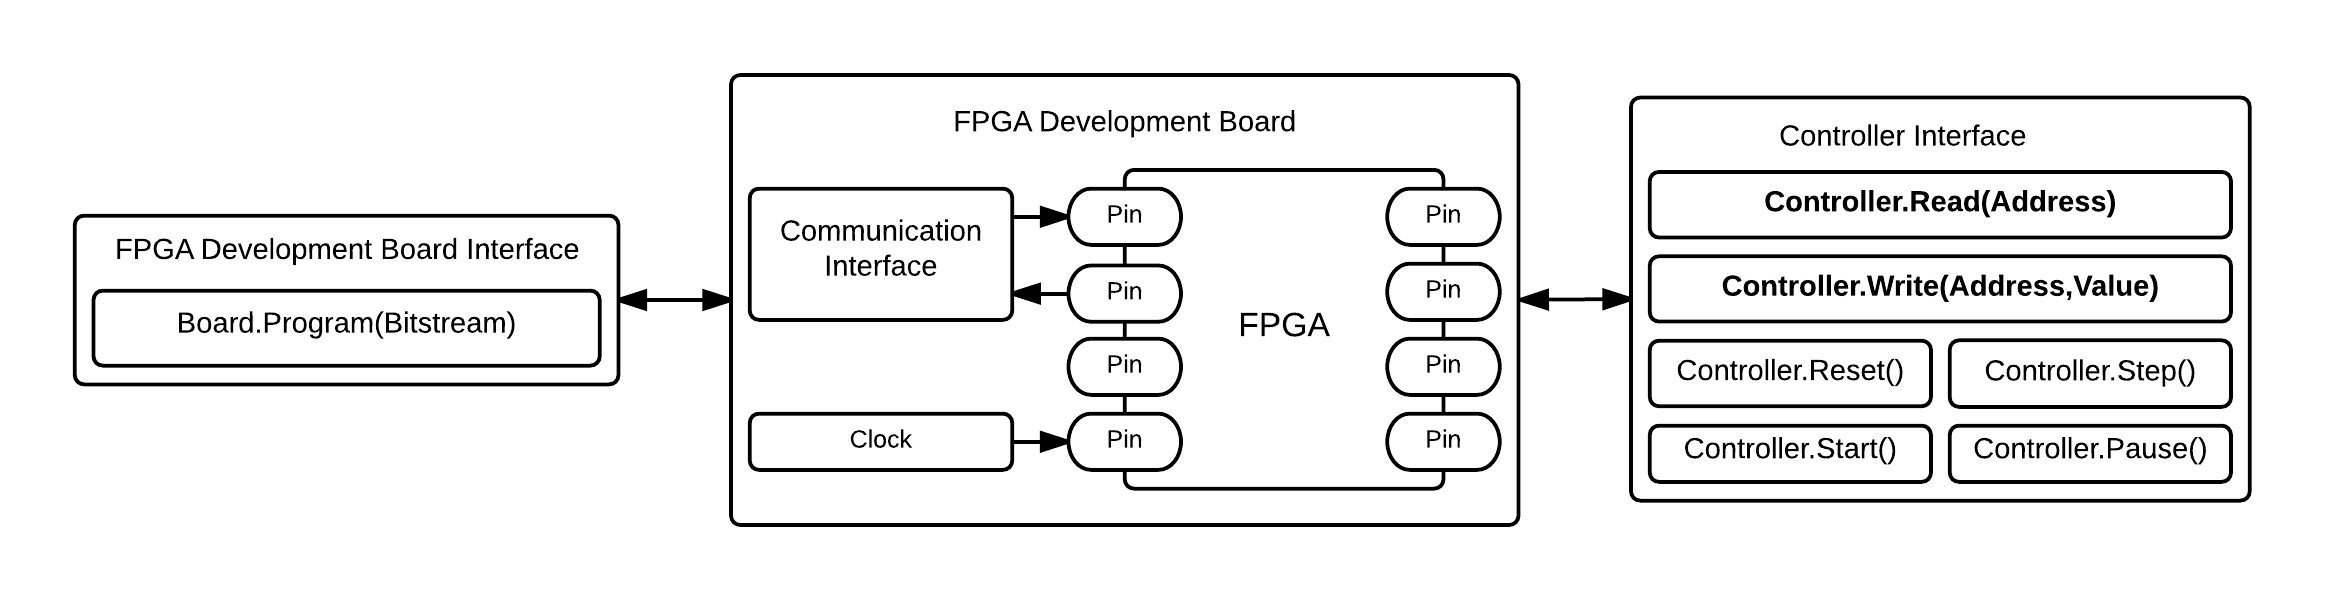
\includegraphics[width=\textwidth]{img/overview-abstract}
\end{figure}
\begin{figure}[h]
    \centering
    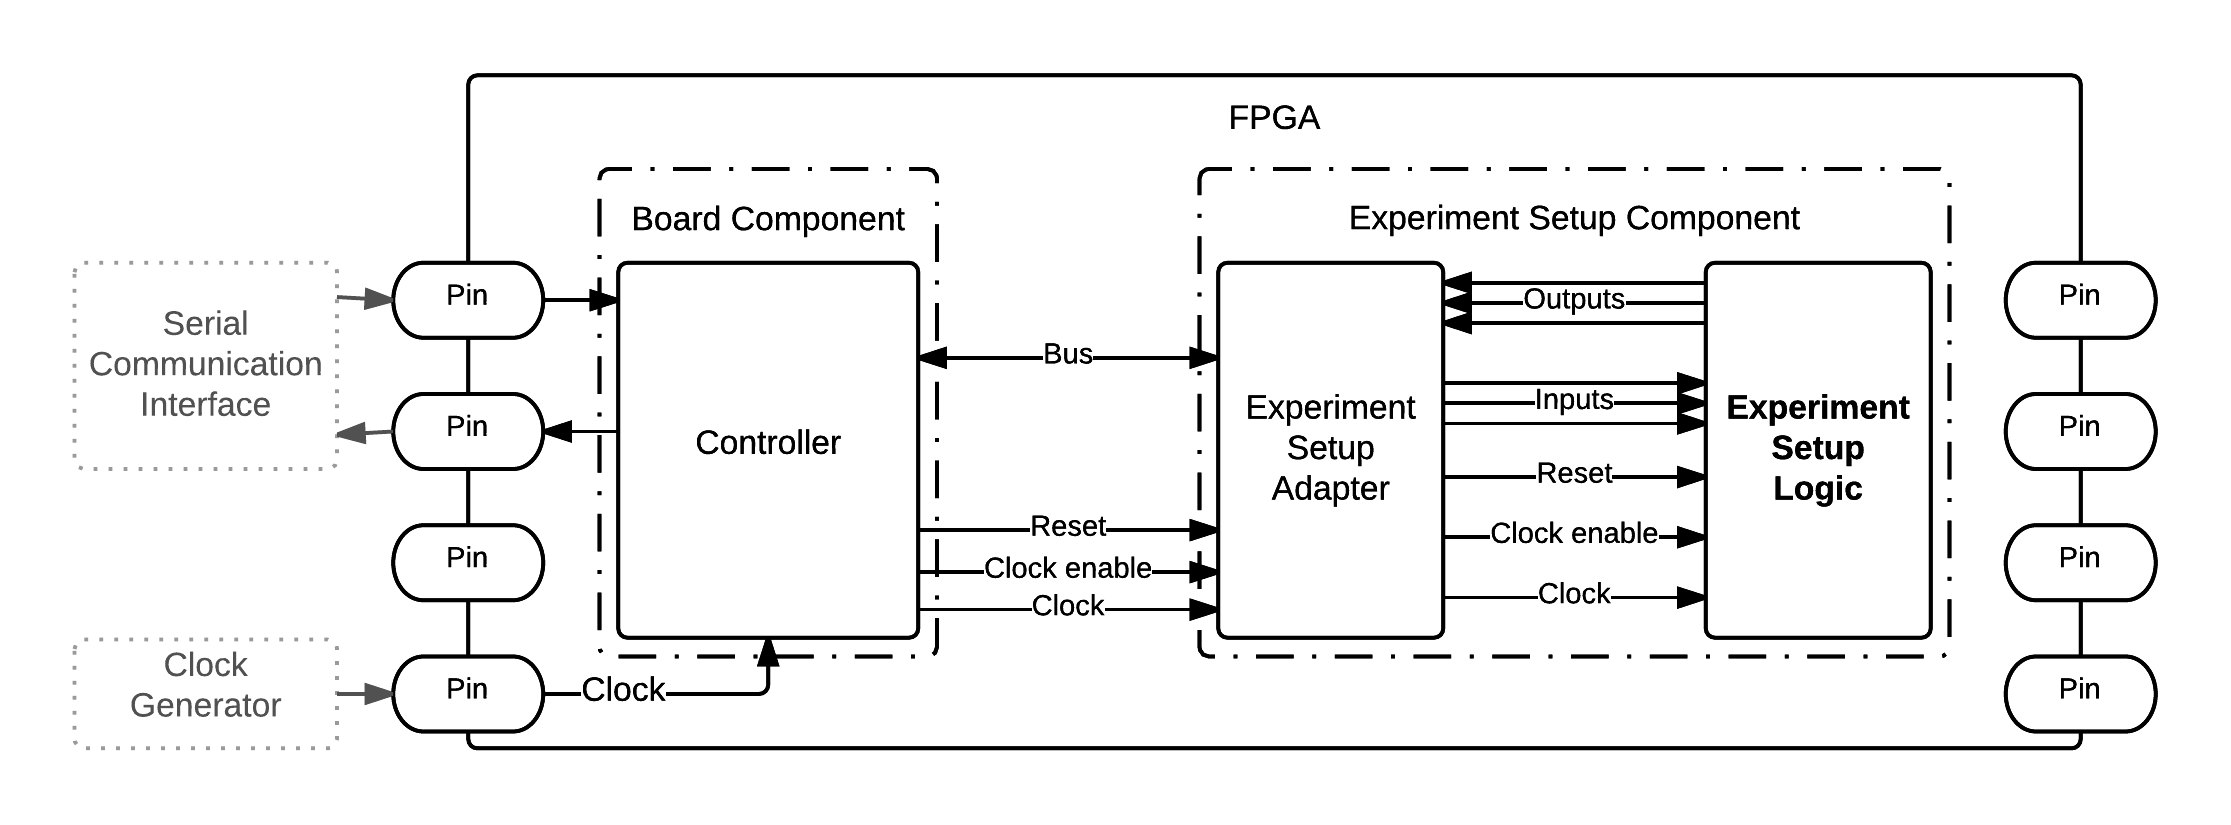
\includegraphics[width=\textwidth]{img/fpga-abstract}
\end{figure}
\end{frame}

\begin{frame}{Model: Generalisatie koppelingen}
\begin{figure}[h]
    \centering
    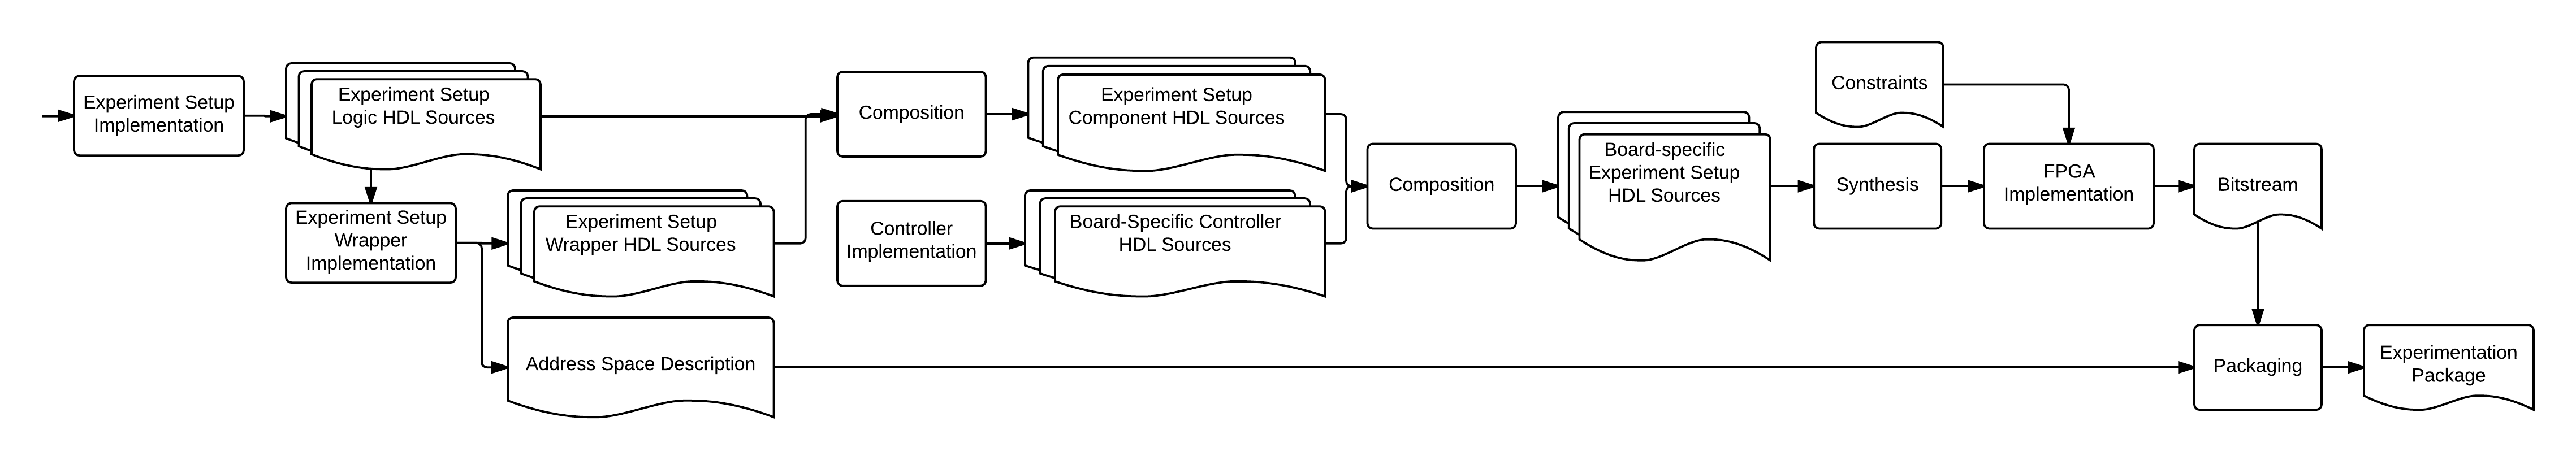
\includegraphics[width=\textwidth]{img/processes-abstract-development}
\end{figure}
\end{frame}


\subsection{Automatisering}
\begin{frame}{Model: Automatisering ontwikkelproces}
\begin{enumerate}
    \item Ontwikkelen
    \item Inpakken (Wrapping)
    \item Compositie (Composition)
\end{enumerate}

\begin{figure}[h]
    \centering
    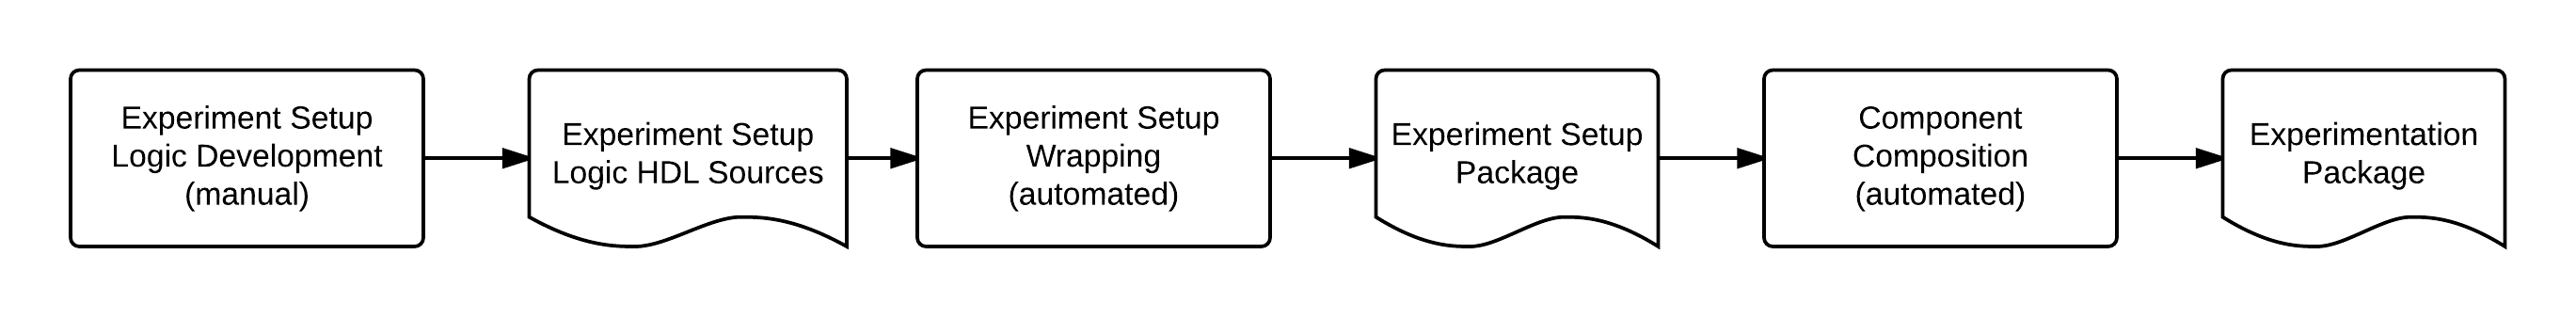
\includegraphics[width=\textwidth]{img/processes-abstract-automation-overview}
\end{figure}

\end{frame}



% Placing a * after \section means it will not show in the
% outline or table of contents.
\section{Resultaten}

\subsection{Implementatie}
\begin{frame}{Implementatie}{Besturende logica\footnote{\url{https://github.com/matthijsbos/fpgaedu-nexys4-python}} (Controller)}
\begin{figure}[h]
\centering
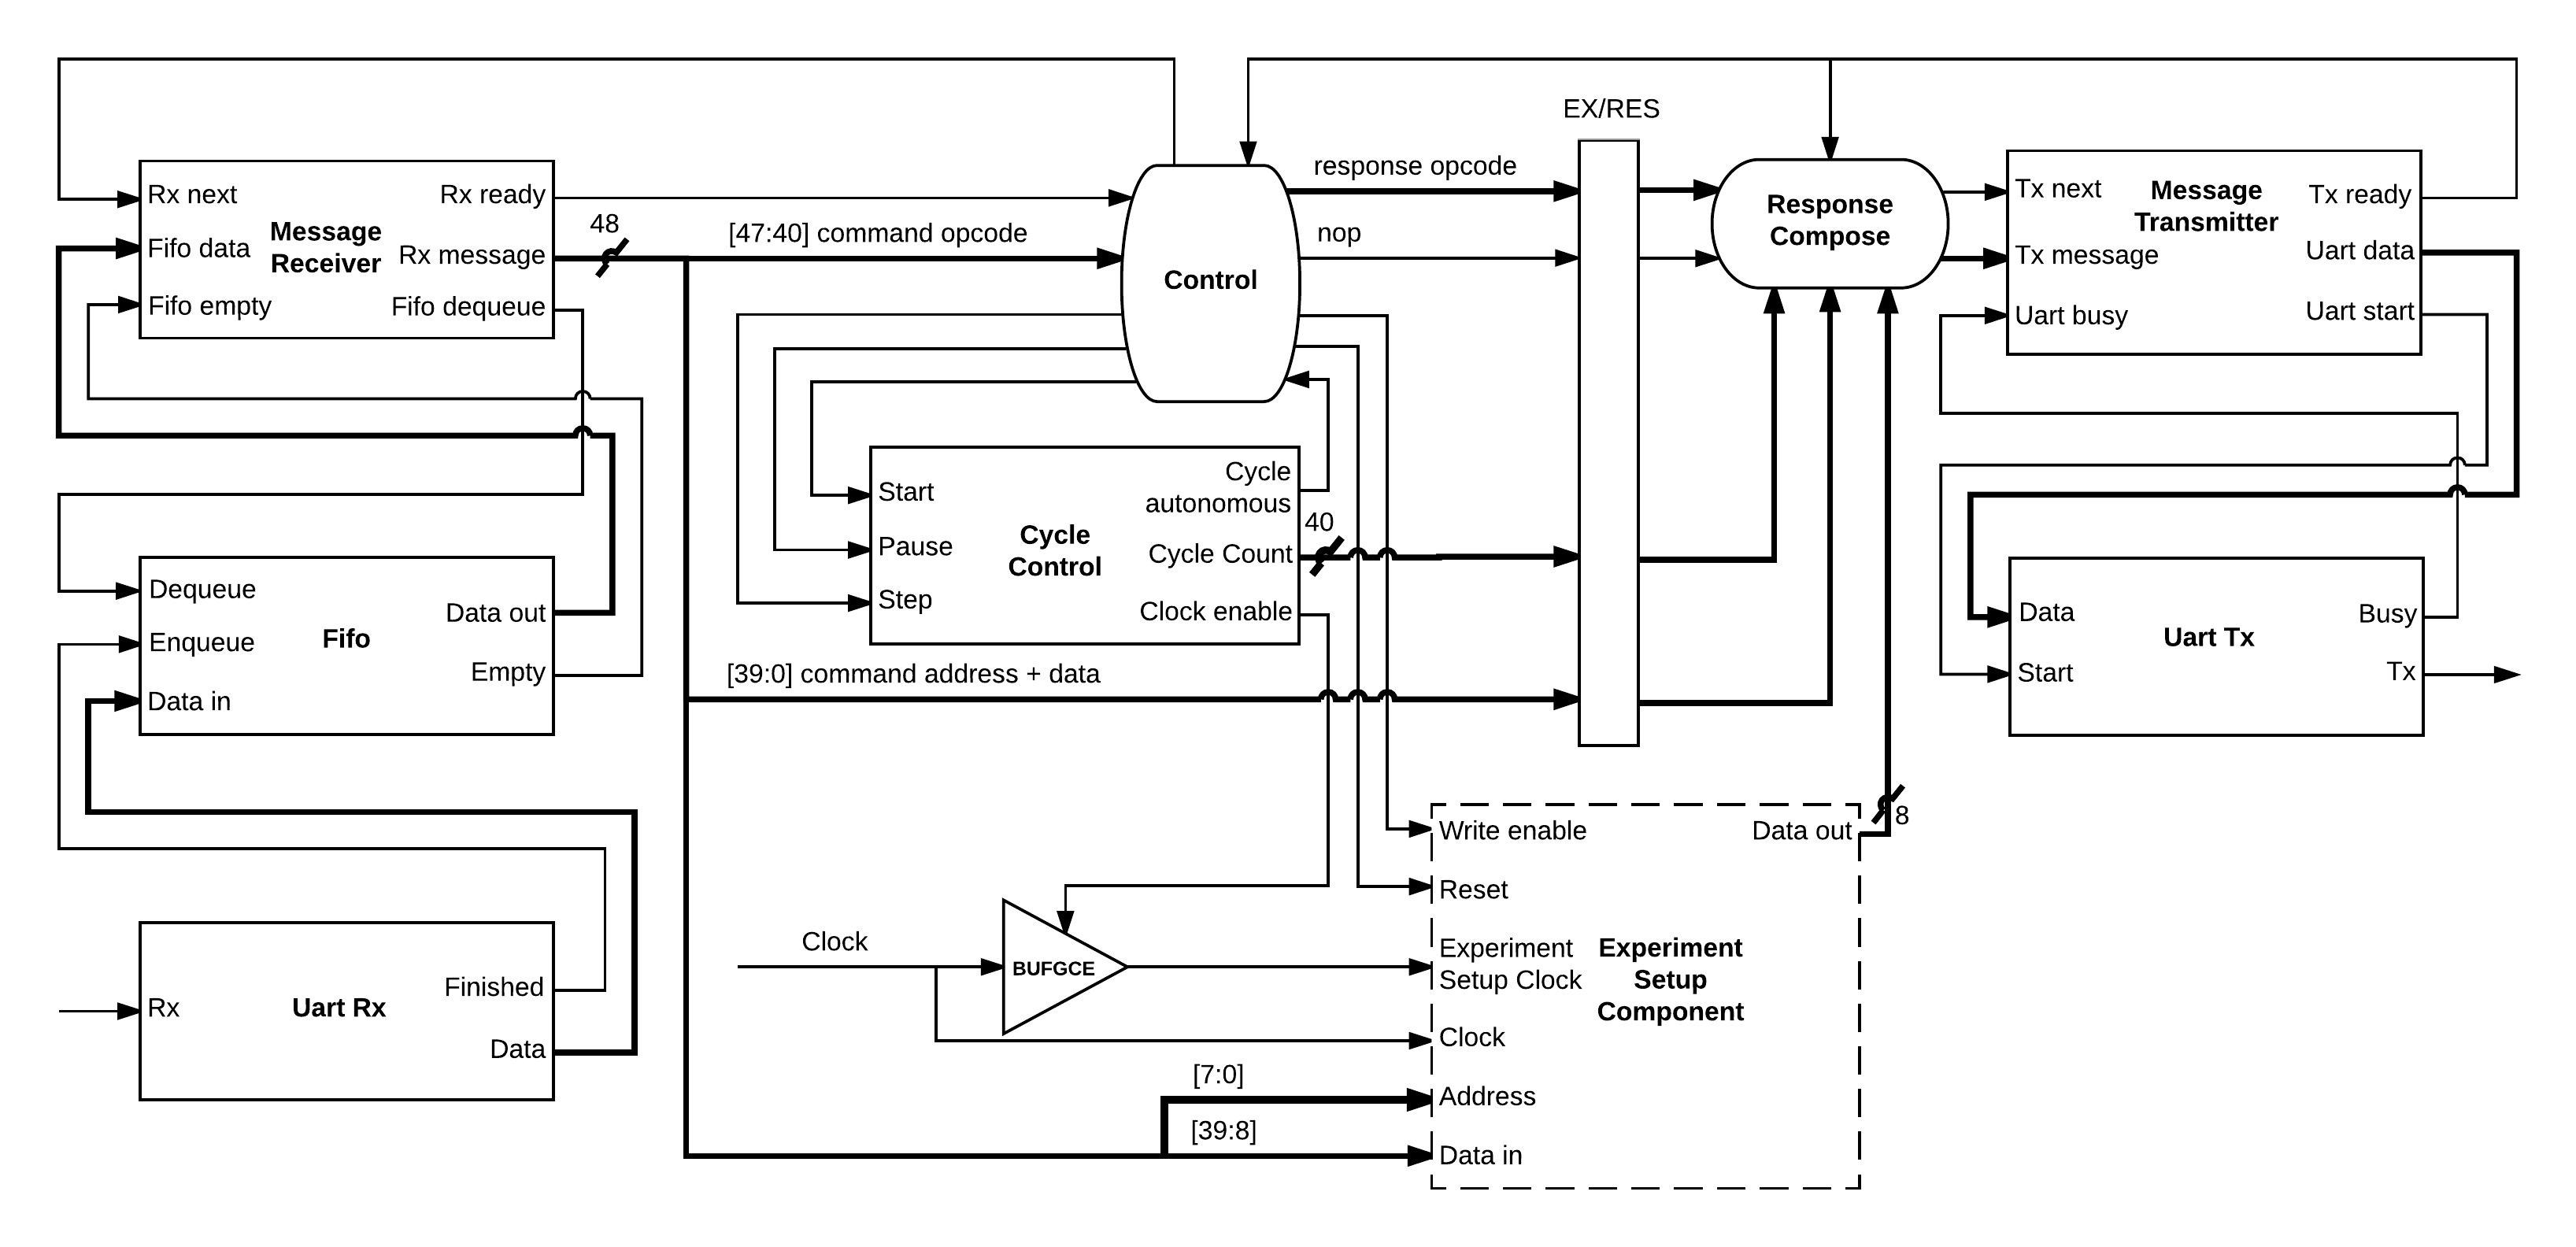
\includegraphics[width=\textwidth]{img/controller-architecture}
\end{figure}

\end{frame}


\begin{frame}{Implementatie}{Automatisering ontwikkelproces\footnote{\url{https://github.com/matthijsbos/fpgaedu-java}}}

\begin{itemize}
    \item Inpakken
        \begin{itemize}
            \item Projectie adresruimte
            \item Genereren logica
        \end{itemize}
        
    \vspace{1em}
    \item Compositie
        \begin{itemize}
            \item Samenvoegen met besturende logica
            \item Geautomatiseerd compileren
        \end{itemize}        
\end{itemize}
\end{frame}

\subsection{Evaluatie}
\begin{frame}{Evaluatie}
\begin{itemize}
    \item Verschillende eenvoudige logische schakelingen
    \item Functionele validatie
    \item Verkorting ontwikkelproces
    \item Vereenvoudiging ontwikkelproces
\end{itemize}
\end{frame}


\section{Slot}

\subsection{Conclusie}
\begin{frame}{Conclusie}

\begin{block}{Adresruimte als generalisatie}

\vspace{1em}

Ontwikkeling

\begin{itemize}
    \item Hergebruik onderdelen architectuur
    \item Afscherming door automatisering
\end{itemize}

\vspace{1em}

Interactie

\begin{itemize}
    \item Afscherming complexiteit FPGA
    \item Experimenteren zonder implementatie
\end{itemize}
\end{block}

\end{frame}

\subsection{Vervolgonderzoek}
\begin{frame}{Vervolgonderzoek}
\begin{itemize}
    \item Praktische toepasbaarheid
    \begin{itemize}
        \item Fysieke interactie ontwikkelbord
        \item PC software
        \item Projectie geheugen elementen
    \end{itemize}
    \vspace{1em}
    \item Andere vakgebieden
\end{itemize}
\end{frame}

\begin{frame}
    
    \begin{center}
    Bedankt voor uw aandacht
    \end{center}
    
\end{frame}


\end{document}


